%% -------------------------------------------------------
% Preamable ---------------------------------------------
%--------------------------------------------------------
%\documentclass[letter,11pt,draft]{article}
\documentclass[letter,11pt]{article}
%-------------------------------------------------------
\usepackage [colorlinks, linkcolor=blue,
  citecolor=magenta, urlcolor=cyan]{hyperref}   % pdf links
% \usepackage {hyperref}
\usepackage{graphicx} % inserting image
\usepackage{setspace} % double/single spacing
\usepackage[top=2cm,right=2cm,bottom=2cm,left=2cm]{geometry} % margins 
\usepackage{amsmath}  %math formulas
\usepackage{array}    %beautiful tables
\usepackage[export]{adjustbox} %aligning images
\usepackage{color,soul} %highlight
\usepackage{subcaption}        %figures with subfigures
\usepackage{amssymb}         %fonts for N, R, ...
\usepackage[font={small}]{caption} %smaller caption fonts
\usepackage[parfill]{parskip}
\usepackage{algorithm,algpseudocode}

\graphicspath{{img/}} %where the images are

\newenvironment{tight_itemize}{
  \begin{itemize}
    \setlength{\itemsep}{0pt}
    \setlength{\parskip}{0pt}
}{\end{itemize}}

\newenvironment{tight_enumerate}{
  \begin{enumerate}
    \setlength{\itemsep}{0pt}
    \setlength{\parskip}{0pt}
}{\end{enumerate}}


\newcommand*\rfrac[2]{{}^{#1}\!/_{#2}}
\newcommand*{\hvec}[1]{\mathbf{#1}}
\newcommand*{\bvec}[1]{\bar{\hvec{#1}}}
\newcommand*{\hmat}[1]{\mathbf{#1}}

% *******************************************************
% Author and title---------------------------------------
% *******************************************************
\title{Final Project, Digital Geometry Processing}
\date{December 2016}
\author{Shayan Hoshyari\\ Student \#: 81382153}

% *******************************************************
% Begin document-----------------------------------------
% *******************************************************
\begin{document}
\pagenumbering{arabic}
\maketitle

% *******************************************************
% ch1- Introduction--------------------------------------
% *******************************************************
\section*{Introduction}

In this project an adaptive surface remesher has been developed based
on the paper \cite{explicit}. An algorithm is proposed to increase the
quality of surface manifold meshes using four fundamental operations,
i.e., edge split, edge collapse, edge flip, and vertex
relocation.

In the first section, strategies are introduced to perform each of the
fundamental operations. Subsequently, the primitive operations are
glued together in the form of a global algorithm. Finally, some
results are presented.

% *******************************************************
% ch2- Primitive Operations -----------------------------
% *******************************************************
\section*{Primitive Strategies}

The concepts of edge collapse, edge flip, edge split, and
vertex relocation are rather straightforward in two
dimensions. However, generalizing them to manifold surfaces needs
extra steps to be taken. In this section we will introduce these core
operations. Namely controlling mesh fidelity, projection of points on
the initial mesh, geodesic polar mapping, Delaunay edge flips, area
based vertex relocation, and Laplacian smoothing.

%% -------------------------------------------------------------------------
\subsection*{Controlling Mesh Fidelity}

In order to prevent deviating from the initial surface we require the
normals of each triangle to be close to the normals at its
vertices. Furthermore, the normals at the vertices should be close to
one another as well. Mathematically, this can be expressed as:

\[\min(N_i,N_j) > \cos(\theta_1) \quad i,j \in T \]
\[\min(N_i,N_T) > \cos(\theta_2) \quad i \in T \]

Where $\theta_1$ and $\theta_2$ are input parameters and are set to
$20$ degrees in this work. $N_i$, and $N_j$ are the normals at any
vertex of the triangle $T$, and $N_T$ is the normal of the triangle
itself. If any of our operations defy these criteria, we simply do not
perform them.

%% -------------------------------------------------------------------------
\subsection*{Projection on the Initial Surface}

All our operations that include vertex insertion or relocation express
the location of a point via the pair $(T,b)$. Where $T$ is a
triangle on the current mesh to whom this new point belongs, and $b$
is the barycentric coordinate of the point on $T$. One strategy is to
choose the location of the point according the current mesh, i.e.,
just interpolate a point on $T$ using $b$. A more advanced strategy
uses overlapping parameterized patches to project the point onto the
original surface. Figure \ref{fig:comp} shows how the former can
deform the surface while the latter preserves the fidelity of the
surface. Both strategies are implemented in this work.

The overlapping parameterized patches work in the following way. First
three triangles on the original mesh that contain vertices of $T$ are
identified. Lets call them $T_o$. Then using the BFS search we create
a patch containing all three members of $T_o$. The patch should be
isomorphic to a disk so we prevent adding triangles that can create
holes. Such a triangle is shown in Figure \ref{fig:hole}. Then the
ears of the patch are trimmed and the patch is mapped to a unit disk
using the CGAL\cite{cgal} library. Then we interpolate the point on the
mapped surface, and find the triangle to whom the interpolated point
belongs, along with its barycentric coordinates. Lets call them $(T_t,
b_t)$. Finally, we use $T_t$ and $b_t$ on the initial mesh to find the
desired location of the point. Figure \ref{fig:patch} shows several
steps of the process.

\begin{figure}
  \centering
  %
  % COMPARISON
  %
  \begin{minipage}{.25\textwidth}
    \centering
    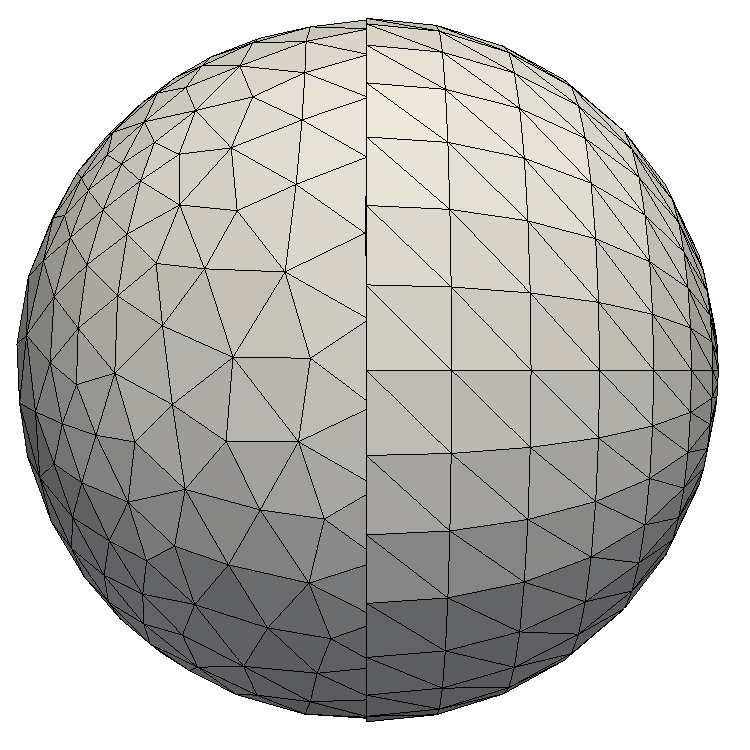
\includegraphics[width=1\linewidth]{../image/sphere_patch.png}
  \end{minipage} 
  % 
  \begin{minipage}{0.25\textwidth}
    \centering
    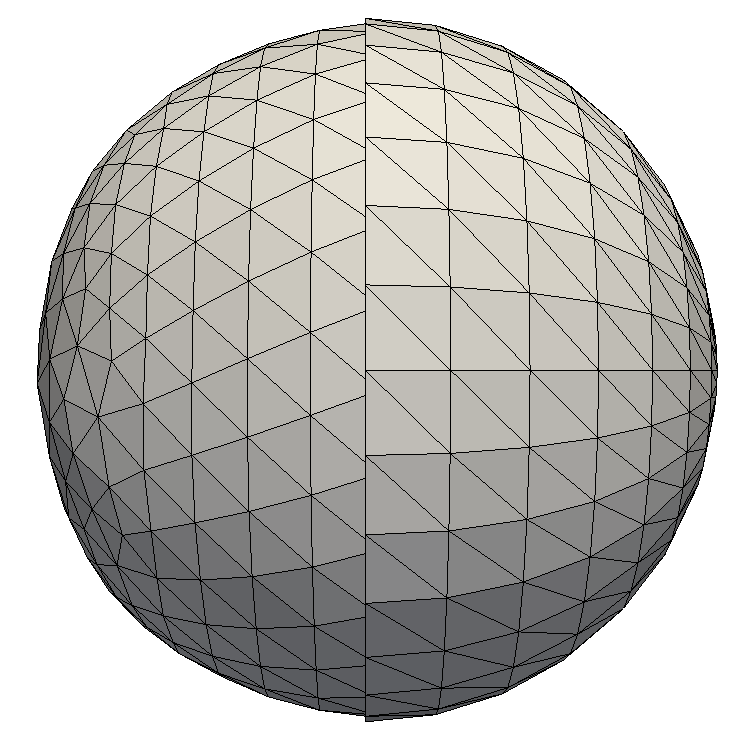
\includegraphics[width=1\linewidth]{../image/sphere_current.png}
  \end{minipage}
  \caption{Comparison of using the current mesh vs. the original mesh
    for vertex insertion and relocation. The left figure shows the
    more advanced overlapping parameterized patches technique which is
    clearly closer to the original surface than the right column which
    uses the current mesh for vertex relocation. The original surface
    is shown for comparison.}
  %
  \label{fig:comp}
  %
  % HOLE
  %
  \vspace{1cm}
  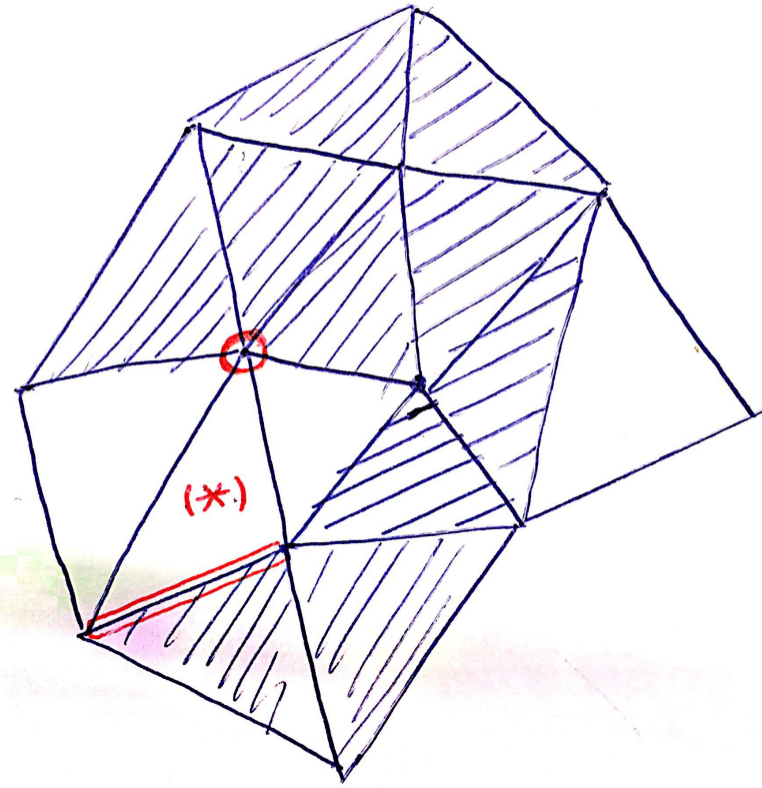
\includegraphics[width=0.25\linewidth]{../image/bfs.png}
  \caption{The starred triangle is an example that should not be
    added to the patch. The dashed triangles are already members of
    the patch. We identify the starred triangle by the fact that it
    only has one neighbor which is inside the patch and a vertex
    which belongs to triangles that are members of the patch.  }
  %
  \label{fig:hole}
  %
  % PATCH
  %
  \vspace{1cm}
  \begin{minipage}{.2\textwidth}
    \centering
    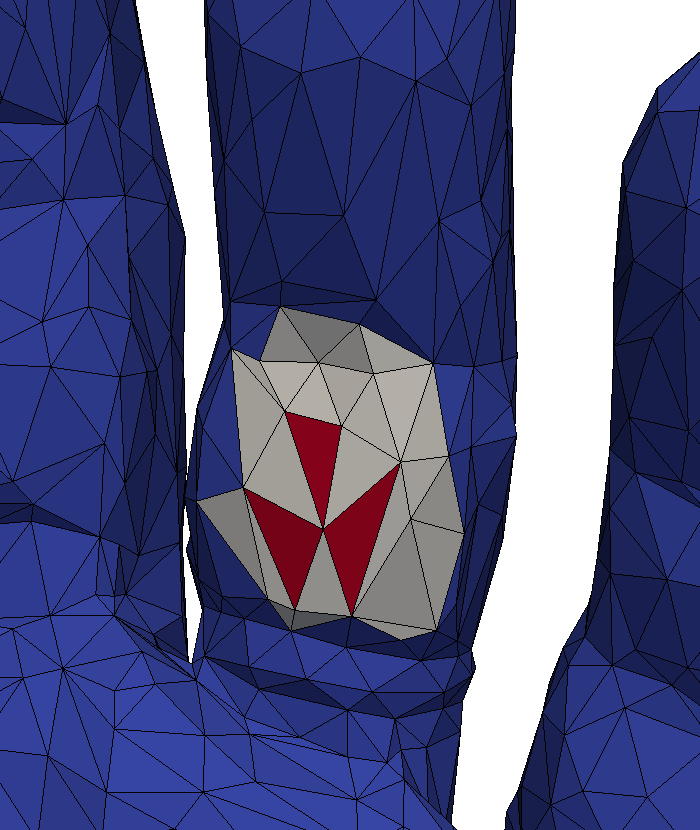
\includegraphics[width=1\linewidth]{../image/patch0.png}
  \end{minipage} 
  % 
  \begin{minipage}{0.2\textwidth}
    \centering
    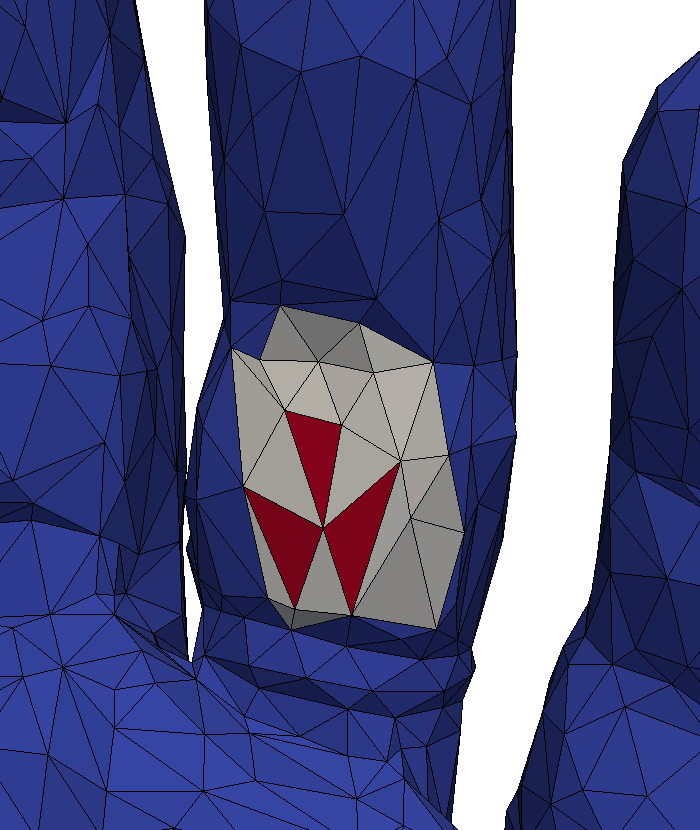
\includegraphics[width=1\linewidth]{../image/patch1.png}
  \end{minipage}
  %
  \begin{minipage}{.2\textwidth}
    \centering
    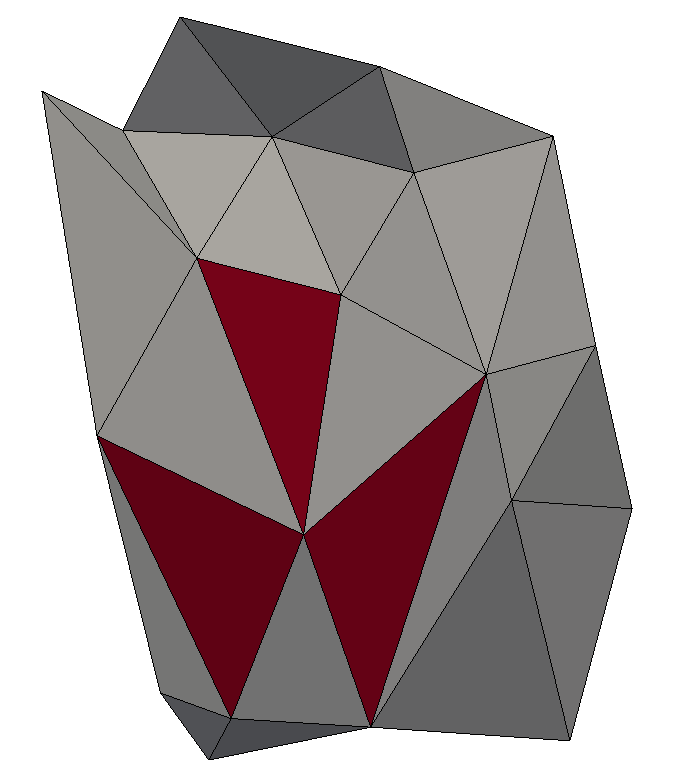
\includegraphics[width=1\linewidth]{../image/patch2.png}
  \end{minipage} 
  % 
  \begin{minipage}{0.2\textwidth}
    \centering
    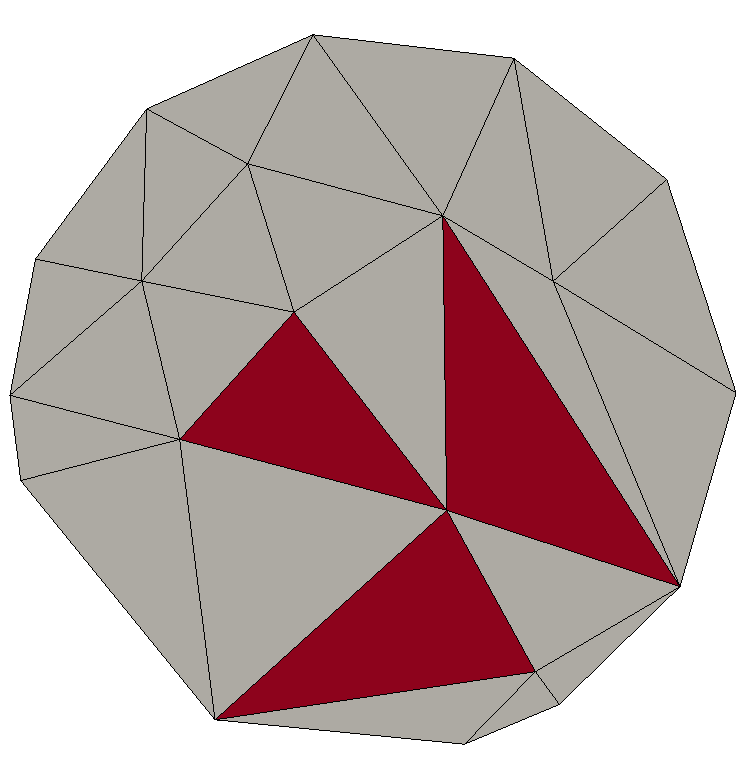
\includegraphics[width=1\linewidth]{../image/patch3.png}
  \end{minipage}
  %
  \caption{Overlapping parameterized patches: The left figure shows
    three triangles $T_o$ on the initial mesh that contain an
    imaginary triangle $T_c$ on the current mesh. Using the BFS search
    a patch is created containing all these three triangles. In the
    second figure the ears of the patch are trimmed. The third figure
    shows an isolated view of the patch. In the fourth figure the
    patch is mapped to a unit disk.}
  %
  \label{fig:patch}
\end{figure}

%% -------------------------------------------------------------------------
\subsection*{Geodesic Polar Mapping}

Delaunay edge flips, Laplacian smoothing, and area based vertex
relocation will all be defined in two dimensions. In order to perform
them on surface meshes we first map the neighborhood of a vertex or
an edge to two dimension, and then perform the operation. In the case
of vertex relocation we use the barycentric coordinate of the mapped
triangle to map the point back to three dimensions.

Figure \ref{fig:geo} shows the schematic of such a mapping. In the case
of an edge one of the triangles is just rotated around the common edge
until both are co-planar. In the case of a vertex we preserve the
length of edges connecting the vertex to the neighboring ones but
scale the angles by a constant factor so that they sum to $2\pi$.

\begin{figure}
  \centering
  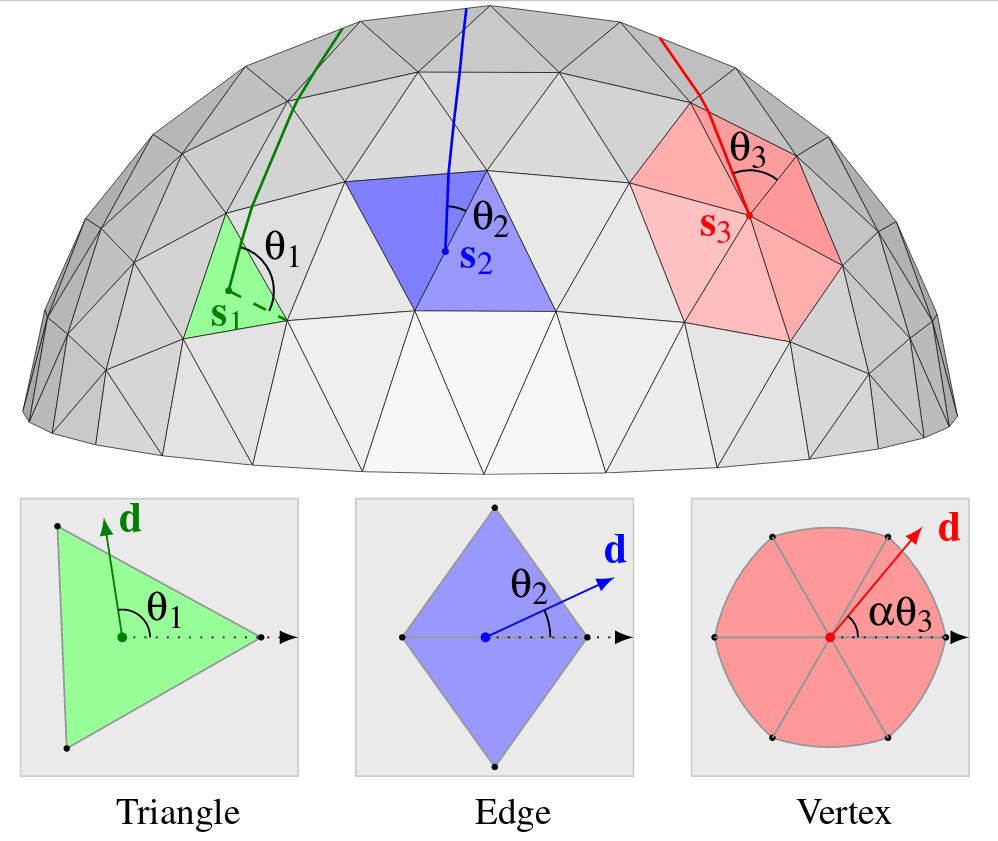
\includegraphics[width=0.4\linewidth]{../image/geodesic.png}
  \caption{Schematic of geodesic polar mapping of the neighborhood of
    an edge or a vertex. The picture is taken from reference \cite{geodesic}.}
  %
  \label{fig:geo}
\end{figure}

%% -------------------------------------------------------------------------
\subsection*{Delaunay Edge Flips}

In order to ensure that all edges are Delaunay in the geodesic polar
mapping sense, we use algorithm \ref{alg:del} taken from \cite{delaunay}.

\begin{algorithm}
  \caption{Delaunay Flips}
  \label{alg:del}
  %
  \begin{algorithmic}[1]
    %
    \State  Push all non-locally interior edges of T on stack and mark them.
    \While {stack is non-empty}
    \State $pq$ = pop()
    \State unmark $pq$
    \If {$pq$ is non-locally Delaunay}
    \State Replace by the edge connecting the respective
    third vertices of the two incident triangles
    \State Push other four edges of the two triangles into the stack if unmarked
    \EndIf
    \EndWhile
    %
  \end{algorithmic}
\end{algorithm}

%% -------------------------------------------------------------------------
\subsection*{Area Based Vertex Relocation}

The area based vertex relocation ensures that the vertices have a
uniform distribution. As noted by algorithm \ref{alg:glu} this
operation has to be followed by Delaunay edge flips. The idea is
pretty simple, for each interior vertex in the mesh we displace it so
that the area of its adjacent triangles are equalized. It reduces to
solving a linear least squares problem in the following form:
\[ \sum ( A_i(x,y) - \mu_i \sum A_i )^2 = 0 \]
Where $A_i$s are the area of the adjacent triangles, and $(x,y)$ is
the location of the vertex. We solve this problem using QR
decomposition from the ``Armadillo'' linear algebra library. The
parameters $\mu_i$ are chosen to be $1$ in this work, but can
generally be used to control the grading of the mesh.

%% -------------------------------------------------------------------------
\subsection*{Laplacian Smoothing}

When a mesh is almost good, this operation can make it ``very
good''. For each vertex in the mesh we displace it to the average
location of its neighbors in the geodesic polar mapped space.

% *******************************************************
% ch2- Combining Algorithm  -----------------------------
% *******************************************************
\section*{Gluing It All Together}

Having all the small pieces working, we will combine them to create
our remesher. First we read a target number of vertices from the
command line switches. If the number of target vertices is more than
the current vertices we start splitting the biggest edge of bad
triangles. In each round of insertion we sort the edges according to
the quality of adjacent triangles, and start splitting the ones with
the worst neighboring triangles. We do not split an edge when any of
its adjacent triangles have been split in the current round, neither
when it is not the biggest edge of any of the adjacent triangles.

If the number of target vertices is less than the current number of
vertices, we do several rounds of edge collapse. Again we sort edges
according to the quality of neighboring triangles. This time we
collapse edges that have higher quality neighbors first. The edge
being collapsed must not be too big compared to the other edges of the
adjacent triangles, neither should any of those triangles have been
collapsed in the same round.

After each round of insertion or edge collapse we do three rounds of
area based vertex relocation followed by Delaunay edge flips.

Our insertion and collapse algorithm is rather naive, especially in
the vertex reduction scheme where we do not do any insertion at all. A
better approach would be to have all triangles in a priority queue,
and smartly do a combination of collapse and insertion to the bad
triangles.

After the desired number vertices have been reached we have the option
to split all edges that are facing obtuse angles. This step should
only be done once, as recursive performance of this action can create
really tiny triangles that can cause numerical problems.

The next step is to perform ten rounds of area based remeshing. In each
round all vertices will be relocated using the area based method three
times followed by Delaunay edge flips. The quality of the mesh is
further enhanced by performing Laplacian smoothing. Algorithm
\ref{alg:glu} concisely reviews all the involved steps.

\begin{algorithm}
  \caption{Gluing the primitive operations together}
  \label{alg:glu}
  %
  \begin{algorithmic}[1]
    
    \While{Target \# of vertices is reached}  
    \State Sort the edges according to ascending/descending adjacent
    triangle quality.
    \State Split/collapse the edges in the mentioned order. 
    \State Do not collapse or split edges that share an adjacent triangle.
    \State Perform 3 rounds of area based vertex relocation.
    \State Perform Dalauany edge flips.
    \EndWhile
    \State Optionally split all edges facing obtuse angles (not recursively).
    \State Do the following 10 times: 3 rounds of area based vertex relocation
    followed by Delaunay edge flips.
    \State Perform 10 rounds of Laplacian smoothing.
    %
  \end{algorithmic}
\end{algorithm}

% *******************************************************
% ch3- Results              -----------------------------
% *******************************************************
\section*{Results}

The performance of the code is evaluated by remeshing five different
geometries. In the first four cases we use insertion to increase the
number of vertices. The selected geometries are a sphere, the cow,
Olliver's Hand, and Nicolo's face, taken from the aim@shape repository.
We insert points via two different criteria, i.e., splitting the
biggest edge of bad triangles, and removing obtuse angles. In the
fifth case we remesh the horse model using edge collapse. To show the
superiority of the overlapping parameterized patches technique, we also
show the results of the current mesh interpolation for the horse case.

Figure \ref{fig:ins_meshes} shows the initial and remeshed models for
insertion cases. Both the insertion for removing obtuse angles, and
splitting biggest edge of bad triangles work pretty well. The flat
shaded remeshed surfaces bear the same pattern as the original ones,
which shows how the method preserves surface fidelity, specifically in
the hand and face geometries. There are some areas like the nose of
the face model that have high initial fidelity error. These areas
cannot be modified properly and are still poor even after remeshing. A
workaround is to smooth out these areas with adaptive subdivision or
PN triangles before starting the remeshing process.

Figure \ref{fig:col_meshes} shows the horse model which is remeshed
via edge collapse. Although our vertex reduction scheme is rather
naive and only collapses edges without insertion, the increase in mesh
quality is still noticeable. We also see how the overlapping
parameterized patches preserve the mesh fidelity, while using the
current mesh to find vertex locations causes the mesh to shrink. The
overlapping patches have only increased the run time by less than
50\%, which shows they are as efficient as they are effective.

Table \ref{tab:perf} shows a summary of the remeshing performance for
each case. The run time of the code is reasonable even up to 20K
vertices, while the percentage of triangles with good minimum angles
increases with inserting further vertices. The vertex reduction
algorithm does not perform as good as the previous cases, as it
only does edge collapse naively without any insertion.
% ---------------------------------------------------------
% TABLE: Remeshed surfaces statistices
% ---------------------------------------------------------
\begin{table}
  \center
  \caption{Remesher performance. Run time and the percentage of triangles with
    different minimum angles are shown. The horse (a) and (b) cases use
    overlapping patches while horse (c) and (d) use interpolation on the
    current mesh.}
  \label{tab:perf}
  \begin{tabular}{*9c}
    %
    \hline
    &&&
    \multicolumn{6}{c}{Percentage of triangles with certain minimum angles} \\
    % 
    Name &Vertex \# &Run Time
    &$0-10$ &$10-20$ &$20-30$ &$30-40$ &$40-50$ &$50-60$ \\
    \hline
    %
    % SPHERE
    %
    Sphere 0 &$482$ &---
    &$0.00$ &$13.33$ &$20.00$ &$26.67$ &$40.00$ &$0.00$ \\
    %
    Sphere a &$930$ &$0.77$ sec
    &$0.00$ &$0.00$ &$0.00$ &$0.00$ &$16.54$ &$83.56$ \\
    %
    Sphere b &$10000$ &$6.76$ sec
    &$0.00$ &$13.33$ &$20.00$ &$0.03$ &$21.95$ &$78.03$ \\
    \hline
    %
    % COW
    %
    Cow 0 &$2904$ &---
    &$3.76$ &$15.23$ &$29.91$ &$30.96$ &$16.25$ &$3.89$ \\
    %
    Cow a &$6000$ &$4.28$ sec
    &$0.47$ &$3.91$ &$9.29$ &$15.54$ &$31.95$ &$38.85$ \\
    %
    Cow b &$20000$ &$14.50$ sec
    &$0.18$ &$1.49$ &$5.15$ &$14.87$ &$31.03$ &$47.28$ \\
    \hline
    %
    % HAND
    %
    Hand 0 &$2531$ &---
    &$0.68$ &$8.94$ &$23.40$ &$31.36$ &$25.66$ &$9.90$ \\
    %
    Hand a &$4320$ &$2.63$ sec
    &$0.17$ &$0.74$ &$2.11$ &$5.86$ &$31.35$ &$59.88$ \\
    %
    Hand b &$20000$ &$15.20$ sec
    &$0.01$ &$0.17$ &$1.21$ &$5.28$ &$27.04$ &$66.29$ \\
    \hline
    %
    % NICOLO
    %
    Face 0 &$2554$ &---
    &$0.76$ &$5.56$ &$18.74$ &$32.11$ &$30.23$ &$12.60$ \\
    %
    Face a &$4129$ &$2.53$ sec
    &$0.26$ &$1.61$ &$4.06$ &$8.27$ &$30.69$ &$55.11$ \\
    %
    Face b &$20000$ &$14.70$ sec
    &$0.03$ &$0.46$ &$2.26$ &$8.82$ &$27.43$ &$60.99$ \\
    \hline
    %
    % HORSE
    %
    Horse 0 &$19851$ &---
    &0.02   &0.44   &6.37  &29.47  &43.00  &20.71 \\
    %
    Horse a &$10000$ &$19.63$ sec
    &0.03 &0.38  &1.40  &4.17  &28.23  &65.79  \\
    %
    Horse b &$5000$ &$16.02$ sec
    &0.09   &1.18   &4.64   &10.59  &31.73   &51.77 \\
    %
    Horse c &$10000$ &$14.60$ sec
    &0.04 &0.28 &0.77 &1.68 &25.50 &71.75 \\
    %
    Horse d &$50000$ &$10.11$ sec
    &0.14  &0.92 &2.31  &5.00 &28.68  &62.95 \\
    \hline
  \end{tabular}
\end{table}
%----------------------------------------------------------

% ---------------------------------------------------------
% IMG: Remeshed surfaces
% ---------------------------------------------------------
\begin{figure}
  \centering
  %
  % SPHERE
  %
  \begin{minipage}{.30\textwidth}
    \centering
    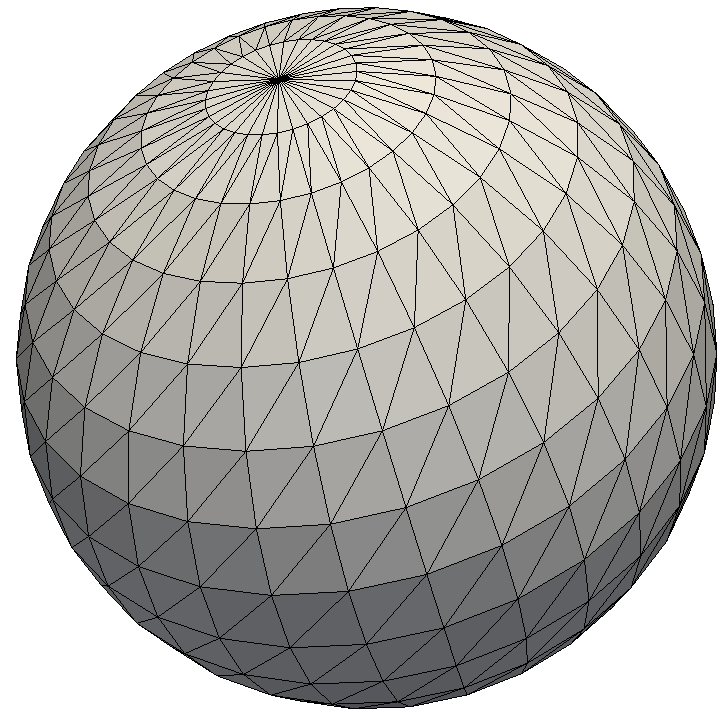
\includegraphics[width=1\linewidth]{../image/sphere_0.png}
  \end{minipage} 
  % 
  \begin{minipage}{0.30\textwidth}
    \centering
    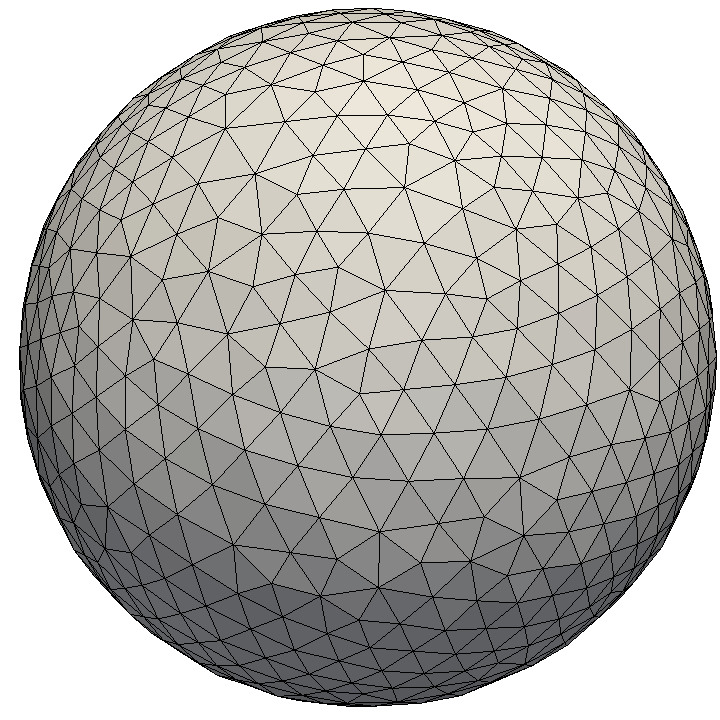
\includegraphics[width=1\linewidth]{../image/sphere_b.png}
  \end{minipage}
  % 
  \begin{minipage}{.30\textwidth}
    \centering
    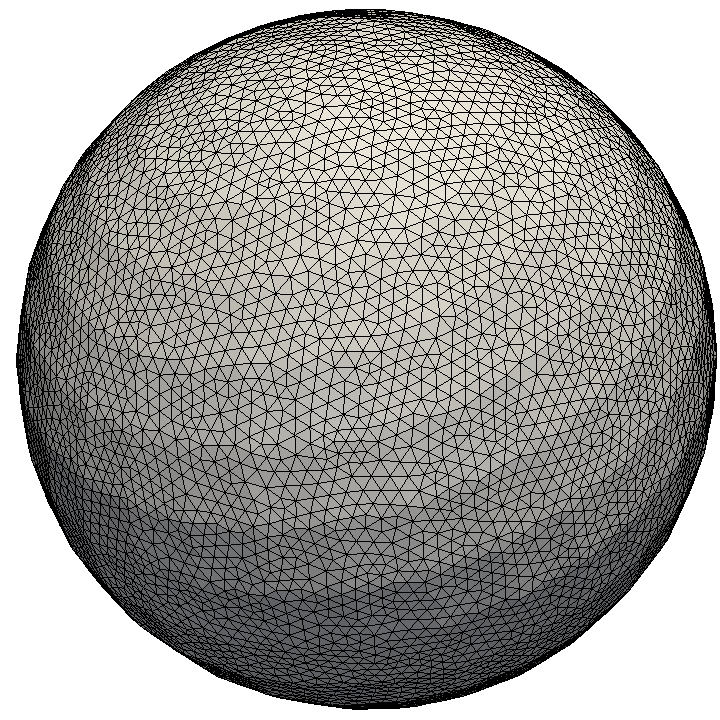
\includegraphics[width=1\linewidth]{../image/sphere_c.png}
  \end{minipage}
  %
  % COW
  %
  \begin{minipage}{.30\textwidth}
    \centering
    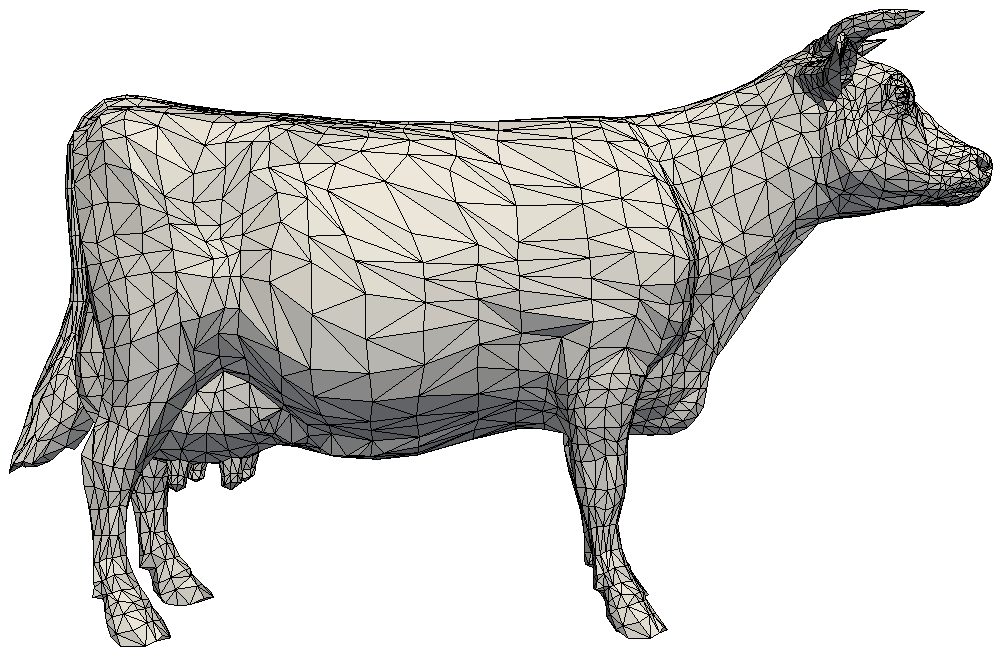
\includegraphics[width=1\linewidth]{../image/cow_0.png}
  \end{minipage} 
  % 
  \begin{minipage}{0.30\textwidth}
    \centering
    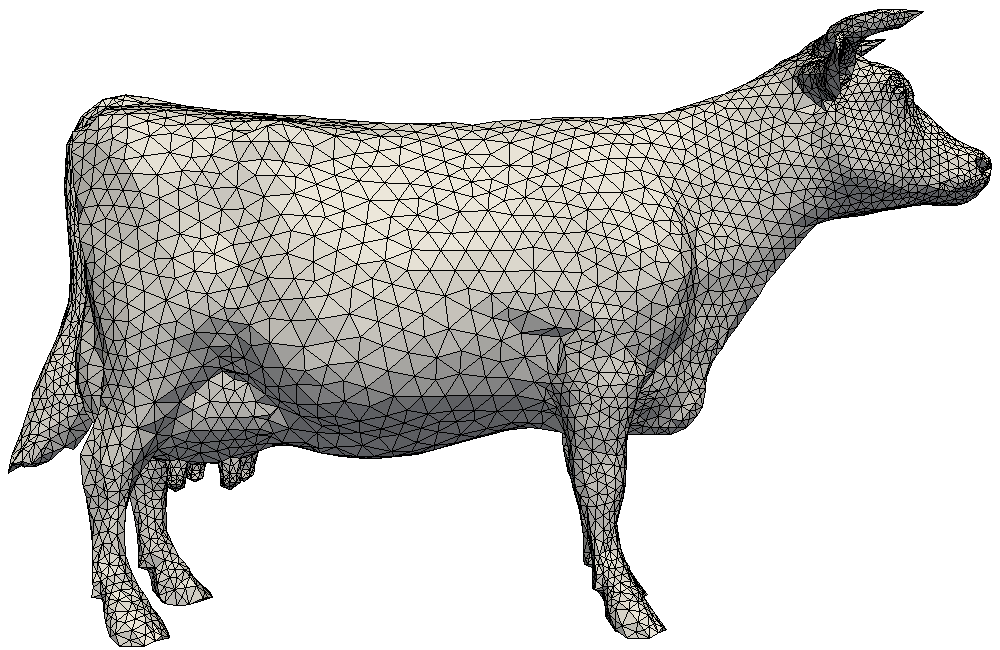
\includegraphics[width=1\linewidth]{../image/cow_b.png}
  \end{minipage}
  % 
  \begin{minipage}{.30\textwidth}
    \centering
    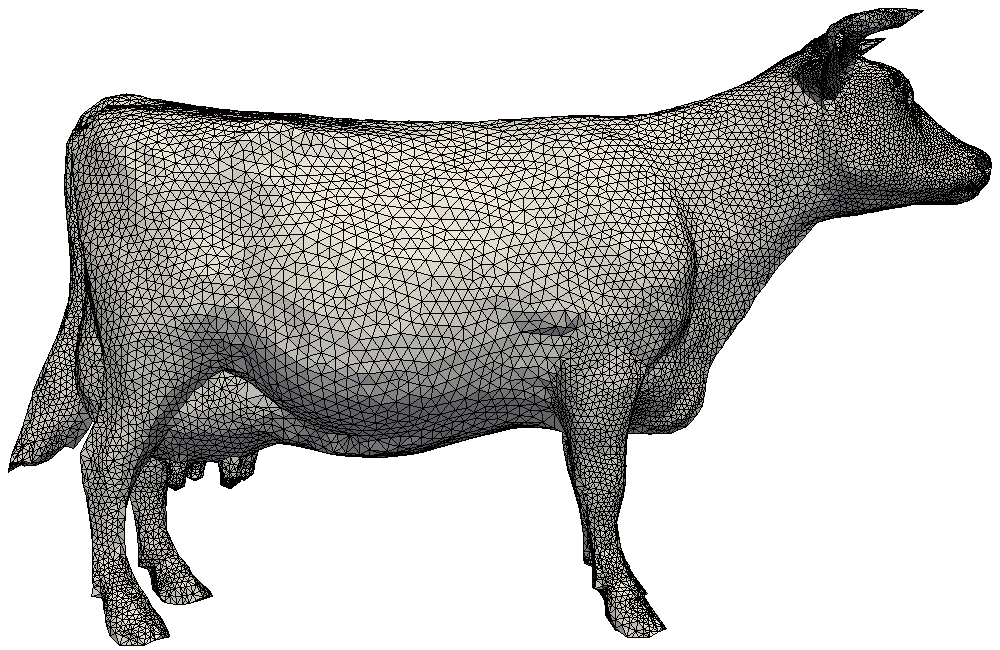
\includegraphics[width=1\linewidth]{../image/cow_c.png}
  \end{minipage} 
  %
  % HAND
  %
  \begin{minipage}{.30\textwidth}
    \centering
    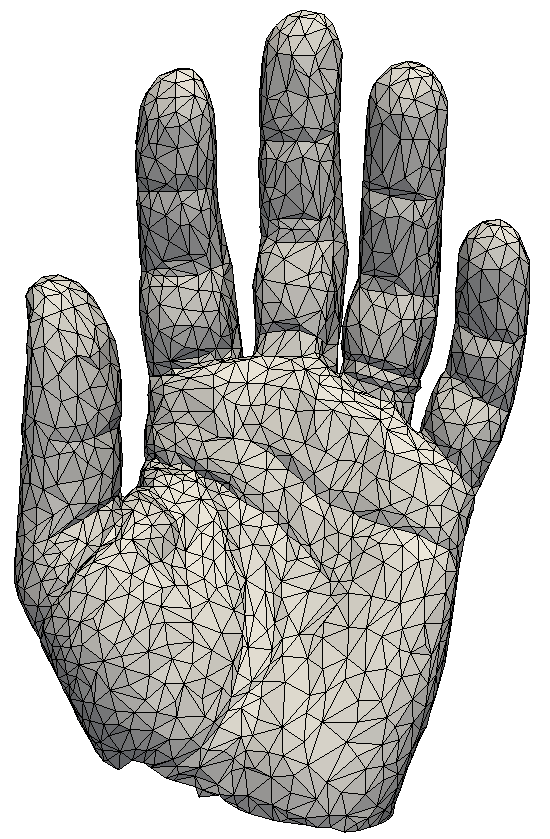
\includegraphics[width=0.7\linewidth]{../image/hand_0.png}
  \end{minipage} 
  % 
  \begin{minipage}{0.30\textwidth}
    \centering
    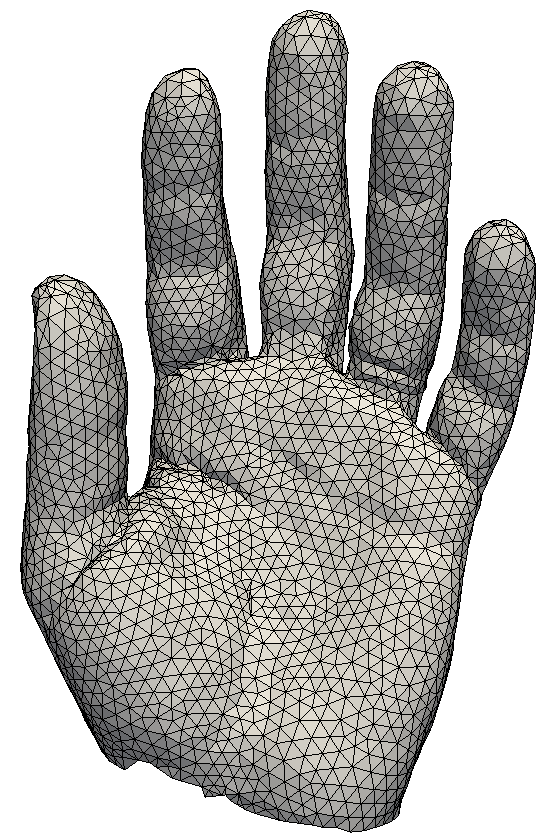
\includegraphics[width=0.7\linewidth]{../image/hand_b.png}
  \end{minipage}
  % 
  \begin{minipage}{.30\textwidth}
    \centering
    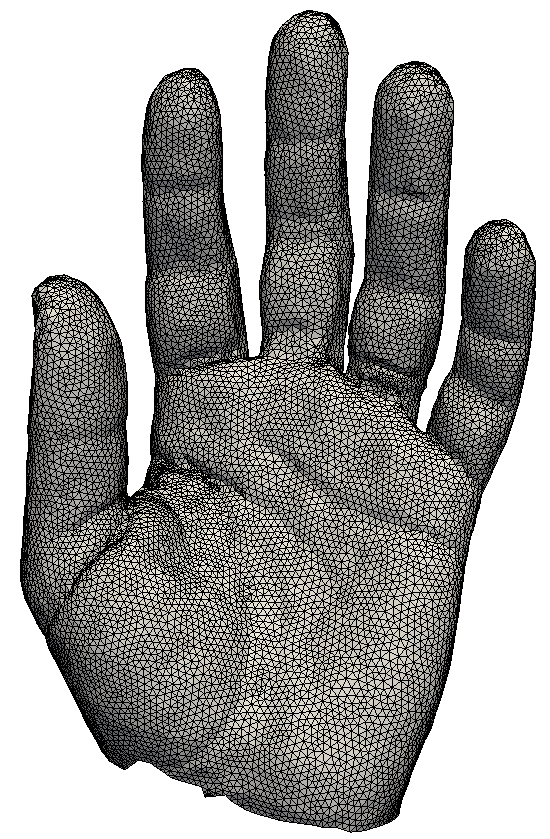
\includegraphics[width=0.7\linewidth]{../image/hand_c.png}
  \end{minipage}
  %
  % NICOLO
  %
  \begin{minipage}{.30\textwidth}
    \centering
    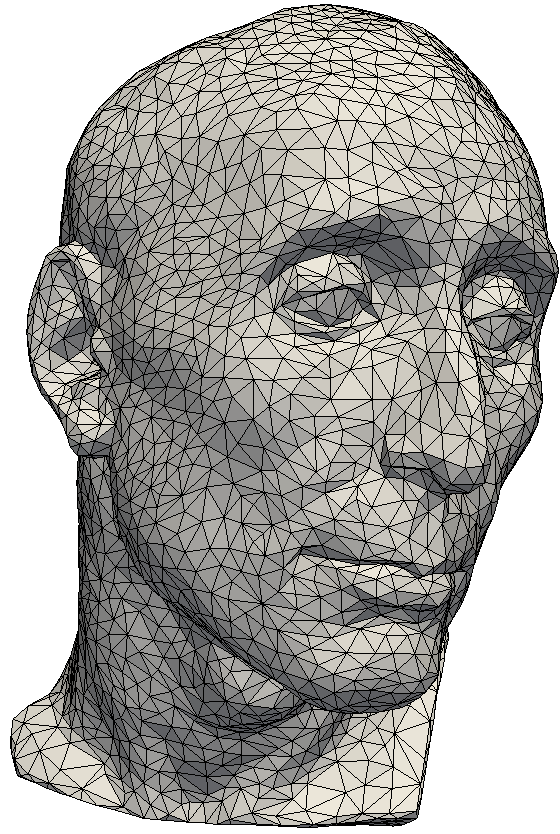
\includegraphics[width=0.7\linewidth]{../image/nicolo_0.png}
  \end{minipage} 
  % 
  \begin{minipage}{0.30\textwidth}
    \centering
    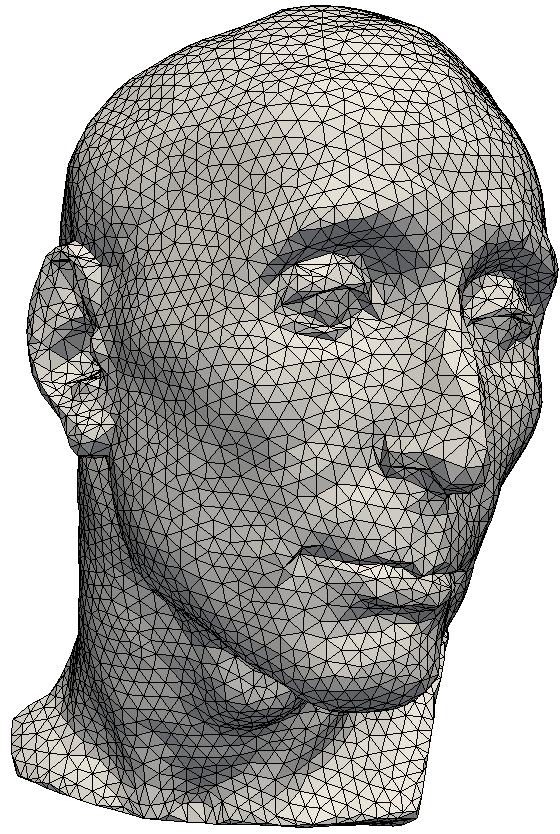
\includegraphics[width=0.7\linewidth]{../image/nicolo_b.png}
  \end{minipage}
  % 
  \begin{minipage}{.30\textwidth}
    \centering
    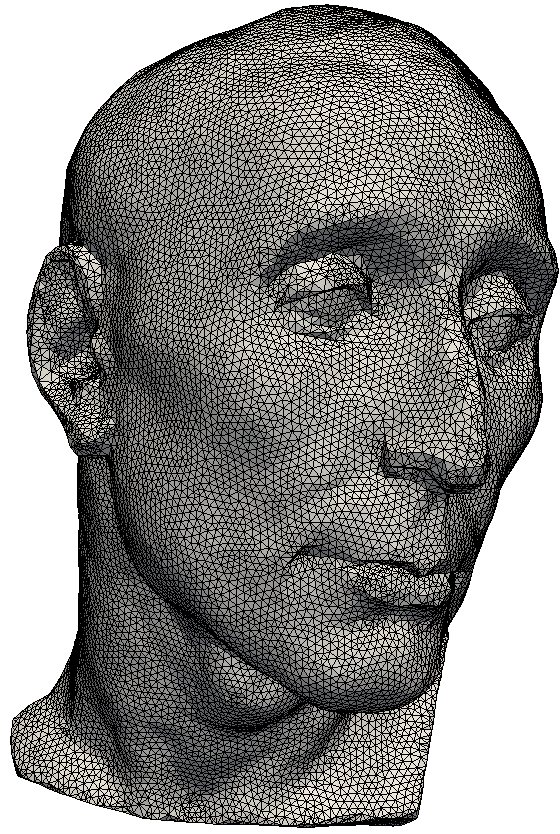
\includegraphics[width=0.7\linewidth]{../image/nicolo_c.png}
  \end{minipage}
  %
  \caption{The models remeshed via insertion. Left column is the
    original model. In the middle column insertion is only performed
    to remove the obtuse angles. In the last column target number of
    vertices is set to 20000.}
  %
  \label{fig:ins_meshes}
\end{figure}
% ---------------------------------------------------------

\begin{figure}
  \centering
  %
  % ORIGINAL
  %
  \begin{minipage}{1\textwidth}
    \centering
    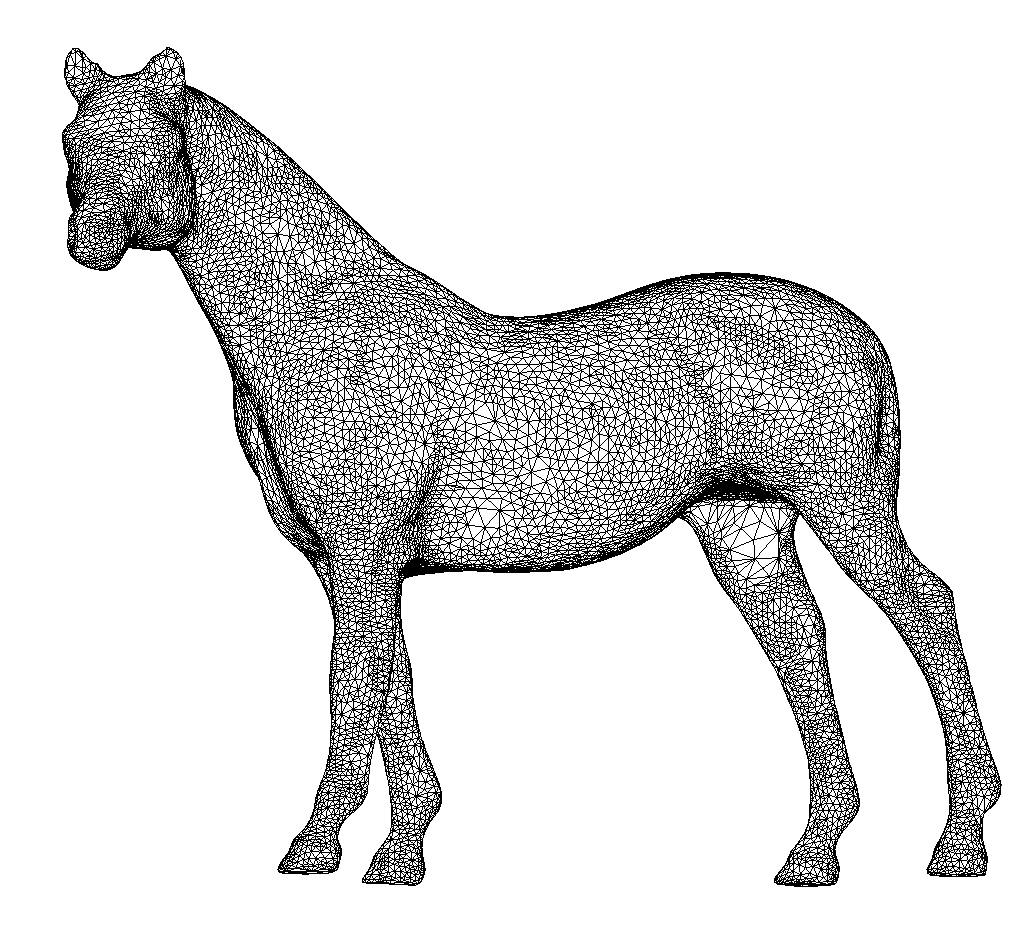
\includegraphics[width=0.50\linewidth]{../image/horse_0.png}
  \end{minipage} 
  % 
  % 10000
  % 
  \begin{minipage}{0.40\textwidth}
    \centering
    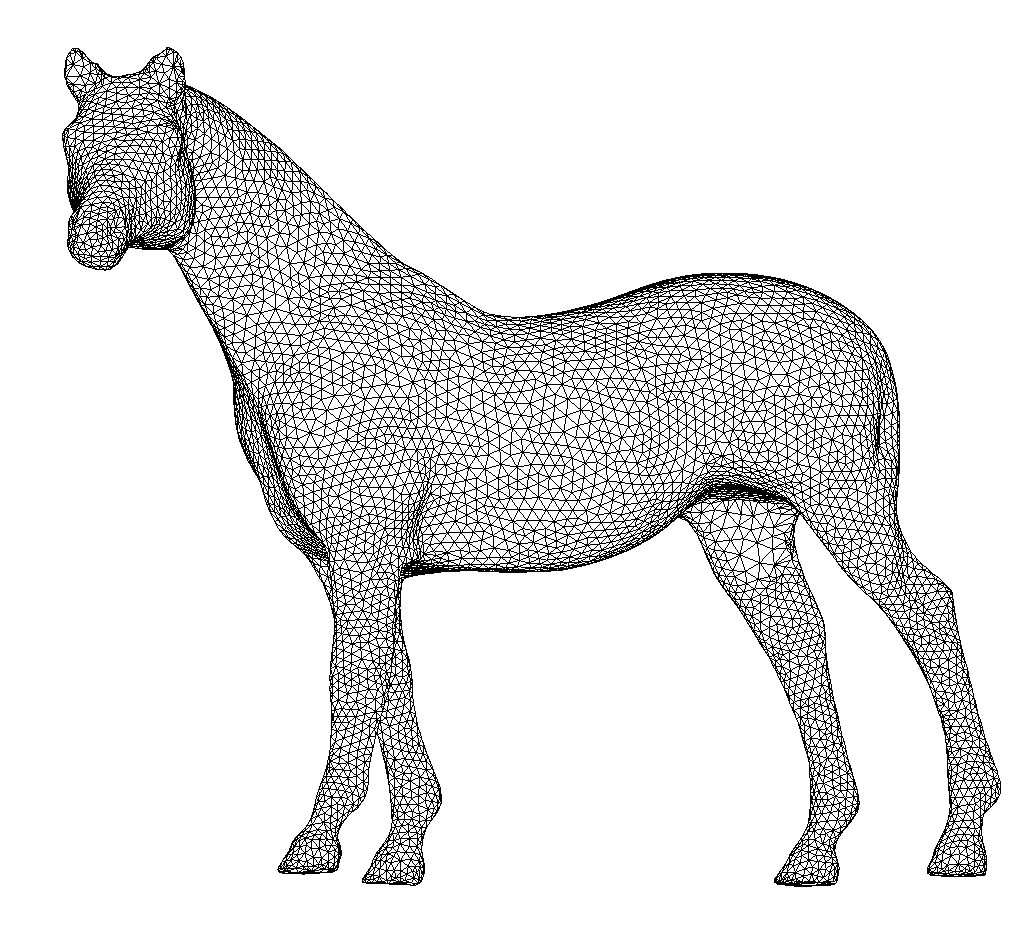
\includegraphics[width=1\linewidth]{../image/horse_a.png}
  \end{minipage}
  % 
  \begin{minipage}{.40\textwidth}
    \centering
    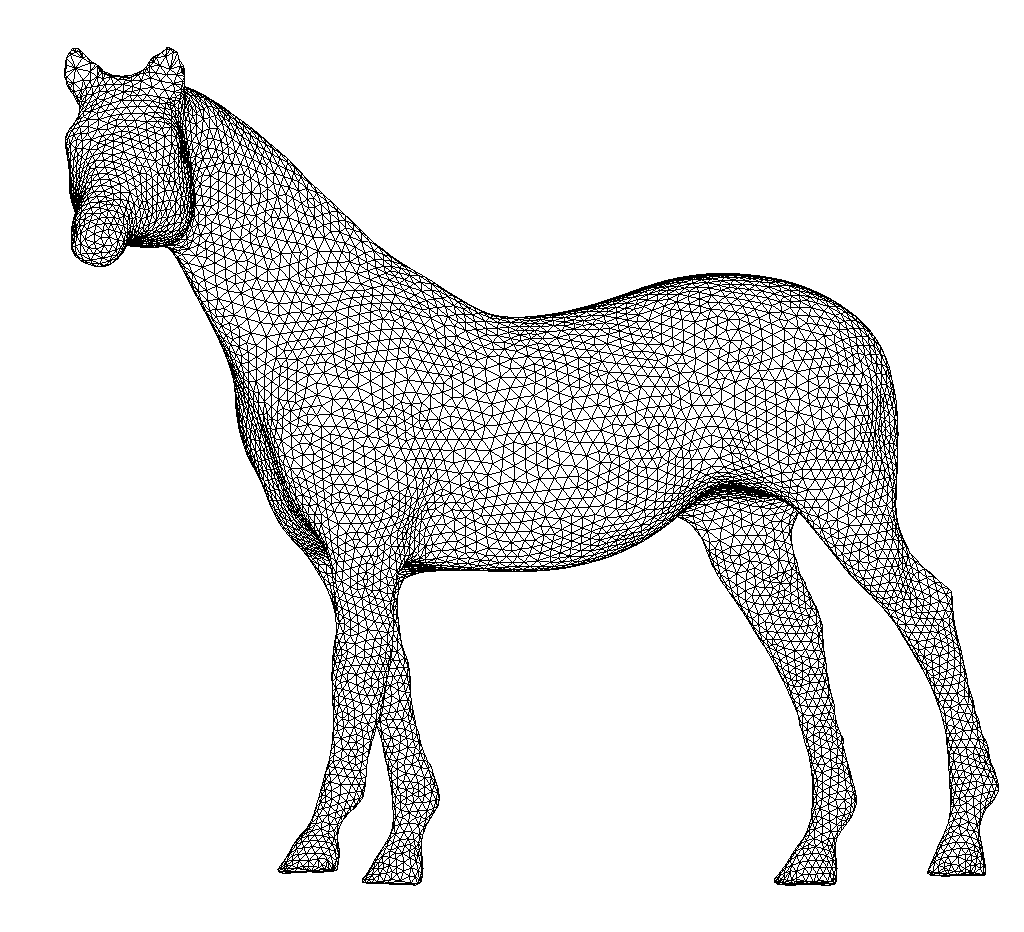
\includegraphics[width=1\linewidth]{../image/horse_c.png}
  \end{minipage}
  %
  % 4000
  %
  \begin{minipage}{.40\textwidth}
    \centering
    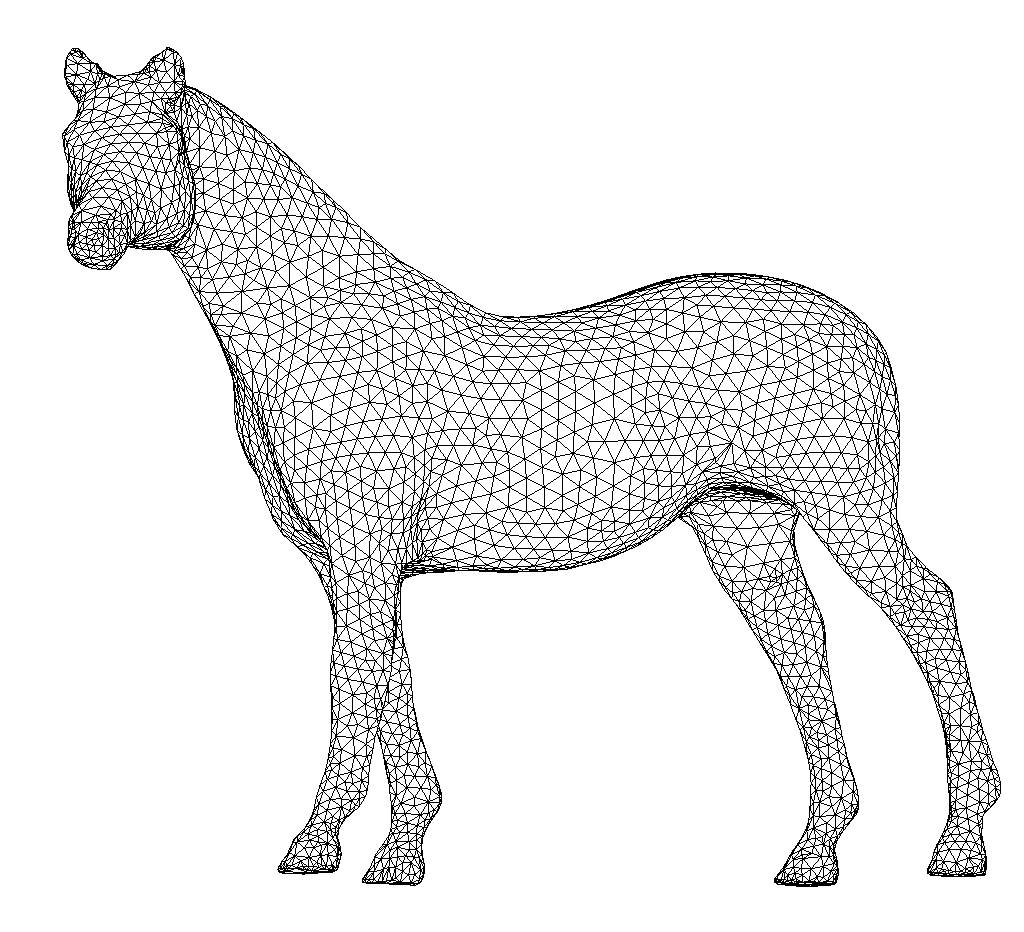
\includegraphics[width=1\linewidth]{../image/horse_b.png}
  \end{minipage} 
  % 
  \begin{minipage}{0.40\textwidth}
    \centering
    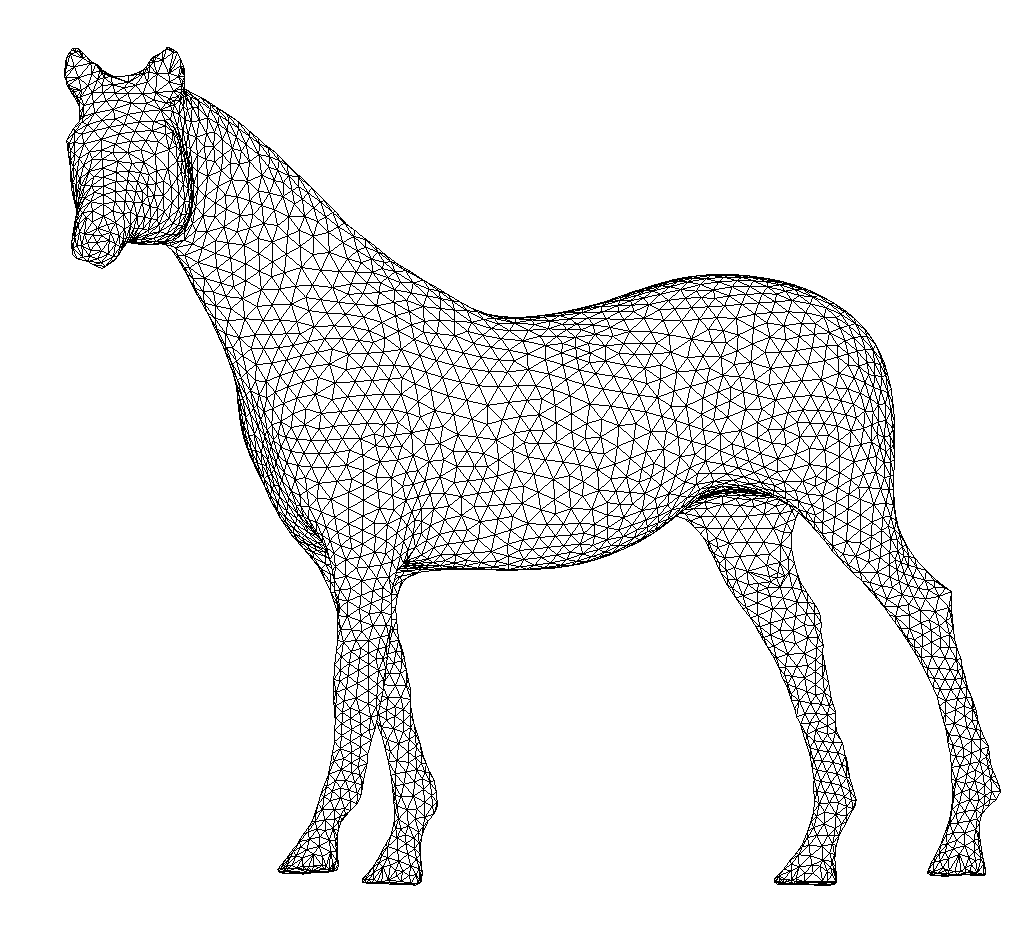
\includegraphics[width=1\linewidth]{../image/horse_d.png}
  \end{minipage}
  %
  \caption{The horse model remeshed via edge collapse. The top figure
    shows the initial mesh. In the left column the new points are
    inserted on the initial surface via the overlapping parameterized
    patches while in the right column the new points are inserted on
    the current mesh. It is clear that the meshes on the right column
    have all shrunk, especially in the mouth and leg areas.}
  %
  \label{fig:col_meshes}
\end{figure}


% *******************************************************
% ch3- Conclusions          -----------------------------
% *******************************************************
\section*{Conclusion}

In this project an adaptive remesher was developed based on the
strategies introduced in the paper \cite{explicit}. Primitive
operations such as edge split, edge collapse, edge flip, and vertex
relocation were performed to increase the quality of the manifold
surface.  As most of the primitive operations are defined in
two-dimensions we used the geodesic polar mapping to map the adjacency
of each vertex or edge into two-dimensions. To ensure the fidelity of
the final surface, two fidelity error criteria were introduced based
on the vertex and triangle normals. Any operation that defies them
should not be performed. Furthermore, the parameterization of
overlapping patches was used in order to project the relocated or
inserted vertices to the original surface. Finally, in order to
evaluate the performance of the code several models were remeshed and
the results were presented.

There are several ways to improve the performance of the
code. Firstly, the initial areas that have high fidelity errors can be
smoothed out before remeshing the surface. Similarly, curved surfaces
such as PN triangles can be used for presenting the initial surface in
order to have smoother remeshed results. Another potential improvement
would be to do edge split and collapse in a smarter way, such as
keeping a priority queue and a criterion to decide whether to collapse
or to split an edge of the worst triangle. Furthermore, feature edges
can be used where the normals are duplicated on each feature
vertex. This allows remeshing of faceted surfaces, such as a cylinder
or a cube. Curvature sensitive triangle size grading can also improve
the quality of the final meshes considerably.

% -------------------------------------------------------
% bibliography-------------------------------------------
%--------------------------------------------------------
\bibliographystyle{ieeetr}
\bibliography{dgp}

\end{document}
